%compare accuracy of the algorithms
%put global feature importance for each algorithm and compare them
%for the best algorithm, put feature importance for each region and compare them


\chapter{Results}

\begin{table}[htbp]
    \centering
    \begin{tabular}{|l|c|c|}
    \hline
    \textbf{Model}           & \textbf{Accuracy} & \textbf{Weighted Average of Precision} \\ \hline
    Logistic Regression & 85.42\%          & 0.73                \\ \hline
    Decision Tree       & 75.97\%          & 0.77              \\ \hline
    Random Forests      & 85.67\%          & 0.83             \\ \hline
    Naïve Bayes         & 85.04\%          & 0.75               \\ \hline
    KNN                 & 83.92\%          & 0.80               \\ \hline
    \end{tabular}
    \caption{Accuracy and Weighted Average of Precision of Different Models}
    \end{table}
    
According to the results shown in the table above, Random Forests and Logistic Regression have the highest accuracy values. However Random Forests has 
higher value on weightes Average of Precision and if the confusion matrixs are compared it can be seen that random forests has higher 
probability of making correct predictions. All those findings makes random forests the best model for this dataset with 84.67\% accuracy. Except Decision Tree, there are not 
significant changes between the algortihms but with accuracy 75.97\% Decision Tree is the worst model for this dataset.
\\
\\
To be able to construct an efficient model and make better understanding on regions' music tastes it is also important to anaylsis importance of
different features of the songs. According to the Random Forest model globally \textit{tempo} is the most important feature while for all the other models 
\textit{dancebility} is the most important feature. This difference can be attributed to the inherent complexity and flexibility of the Random Forest
algorithm, which allows it to capture intricate patterns and interactions in the data that other models may not. Beside having the most important feature globally,
also feature importance is done for each region seperately. This analysis help to understand how the music tastes of different regions are shaped by audio features. 


\newpage
\textbf{Global Feature Importance Extracted From Different Models:}
\begin{figure}[h]
    \centering
    \begin{minipage}{0.45\textwidth}
        \centering
        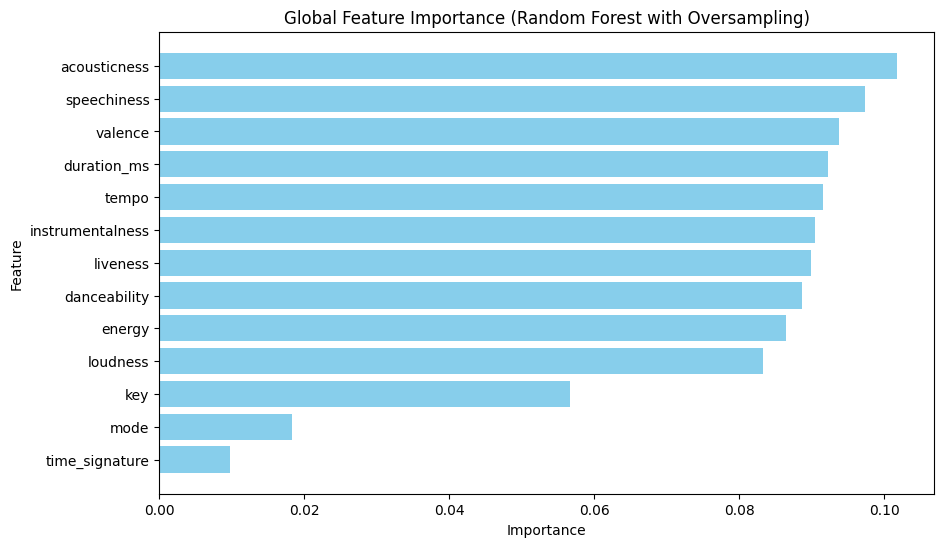
\includegraphics[width=\linewidth]{media/random_forest_feature_imp_global.png}
        \caption{Global Feature Importance Using Random Forests Model}
    \end{minipage}%
    \hspace{0.05\textwidth} % Space between the two figures
    \begin{minipage}{0.45\textwidth}
        \centering
        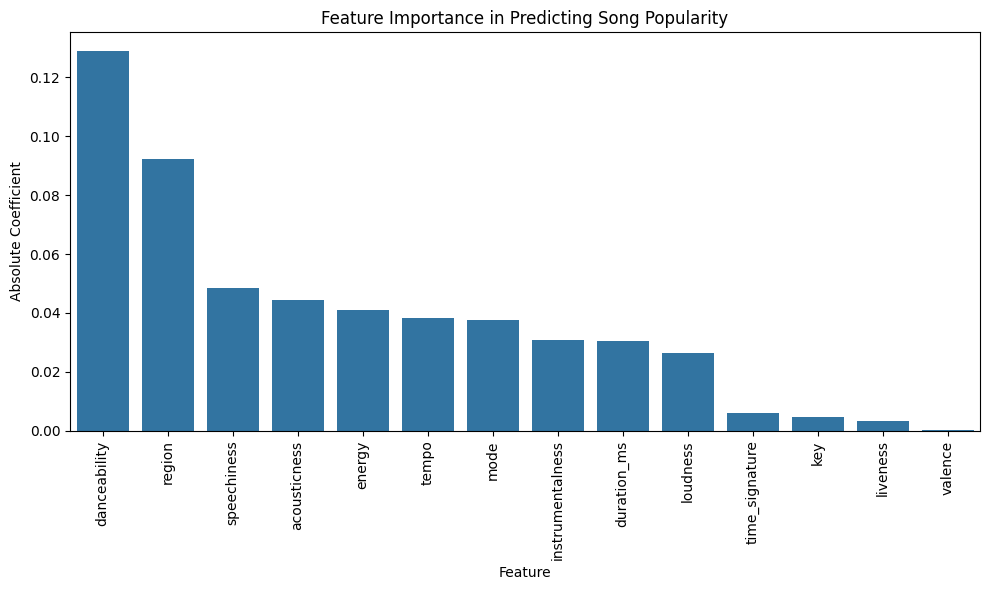
\includegraphics[width=\linewidth]{media/logistic_reg_feature_imp_global.png}
        \caption{Global Feature Importance Using Logistic Regression Model}
    \end{minipage}
\end{figure}
\begin{figure}[h]
    \centering
    \begin{minipage}{0.45\textwidth}
        \centering
        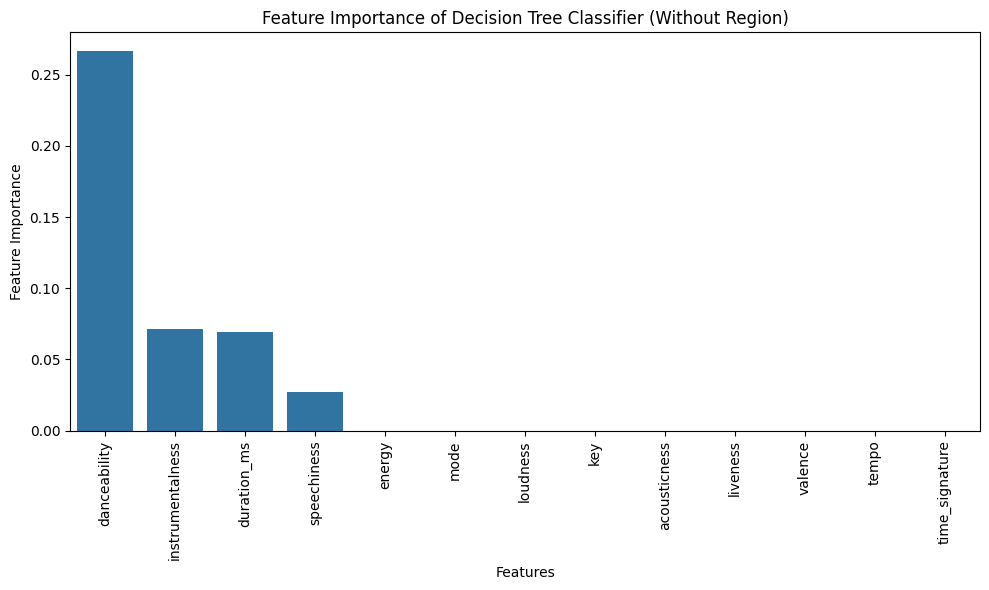
\includegraphics[width=\linewidth]{media/decision_tree_fea_imp_global.png}
        \caption{Global Feature Importance Using Decision Tree Model}
    \end{minipage}%
    \hspace{0.05\textwidth} % Space between the two figures
    \begin{minipage}{0.45\textwidth}
        \centering
        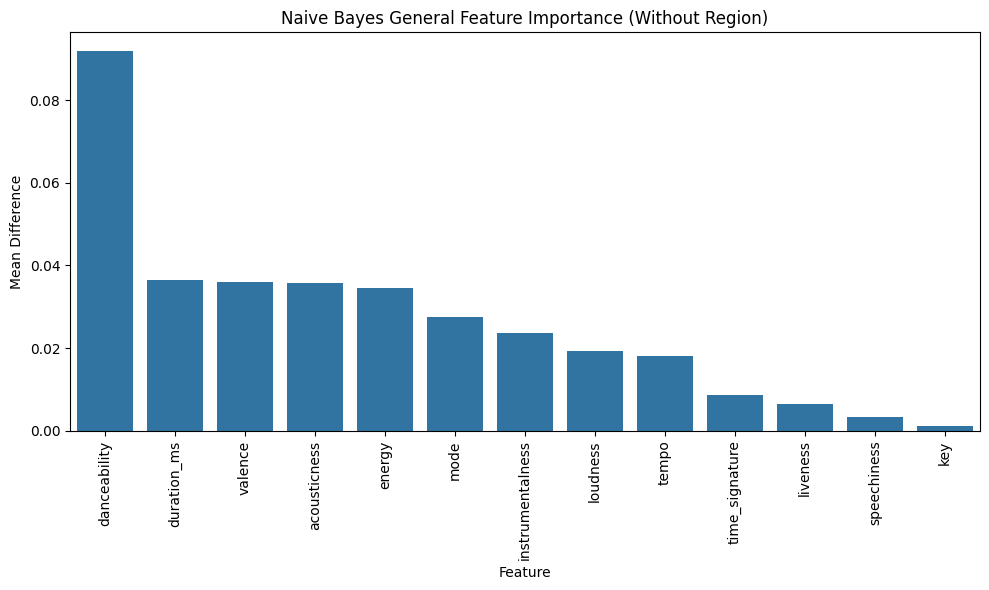
\includegraphics[width=\linewidth]{media/naive_bayes_fea_imp_global.png}
        \caption{Global Feature Importance Using Naive Bayes Model}
    \end{minipage}
\end{figure}
\begin{figure}[h]
    \centering
    \begin{minipage}{0.45\textwidth}
        \centering
        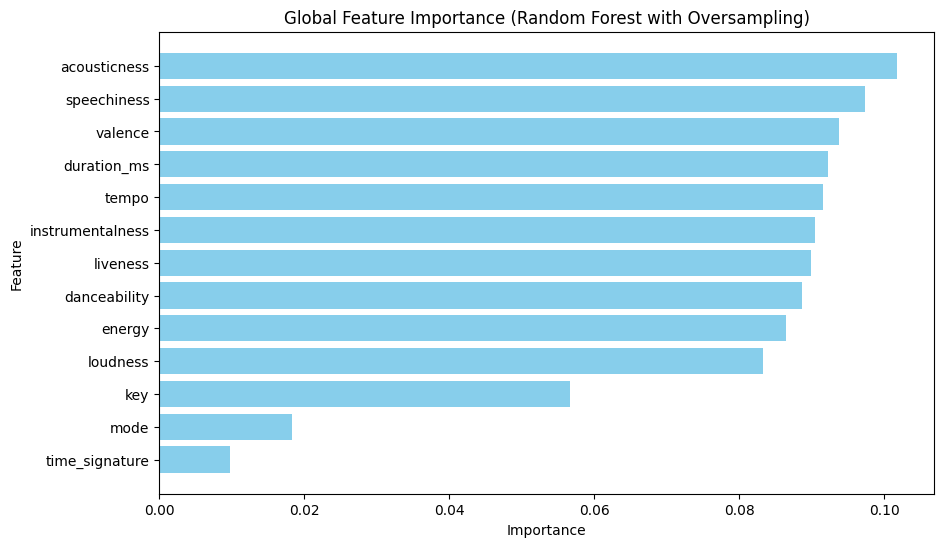
\includegraphics[width=\linewidth]{media/random_forest_feature_imp_global.png} %change it with knn picture
        \caption{Global Feature Importance Using KNN Model}
    \end{minipage}
\end{figure}

\newpage
\textbf{Feature Importance for Each Region Extracted From Random Forest Model:}
\begin{figure}[h]
    \centering
    \begin{minipage}{0.45\textwidth}
        \centering
        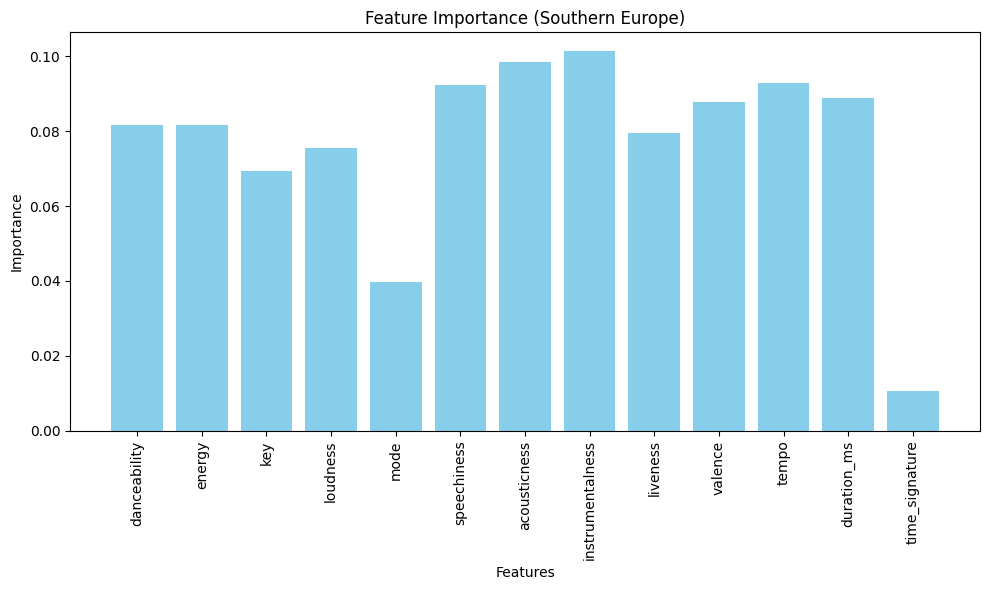
\includegraphics[width=\linewidth]{media/rf_feature_imp_northen_europe.png}
        \caption{Feature Importance in North Europe}
    \end{minipage}%
    \hspace{0.05\textwidth} % Space between the two figures
    \begin{minipage}{0.45\textwidth}
        \centering
        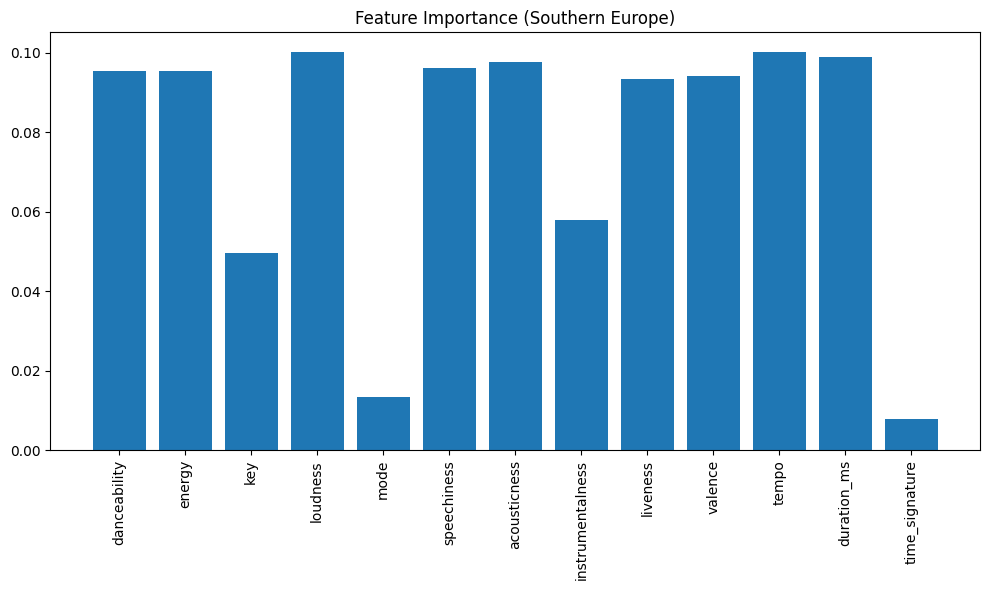
\includegraphics[width=\linewidth]{media/rf_feature_imp_southern_europe.png}
        \caption{Feature Importance in South Europe}
    \end{minipage}
\end{figure}
\begin{figure}[h]
    \centering
    \begin{minipage}{0.45\textwidth}
        \centering
        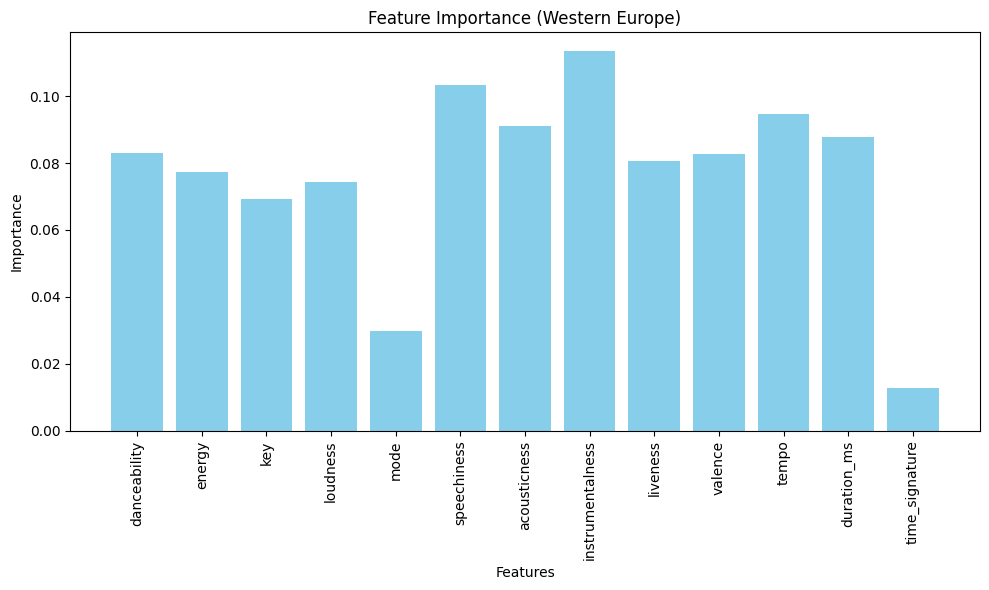
\includegraphics[width=\linewidth]{media/rf_feature_imp_western_europe.png}
        \caption{Feature Importance in Western Europe}
    \end{minipage}%
    \hspace{0.05\textwidth} % Space between the two figures
    \begin{minipage}{0.45\textwidth}
        \centering
        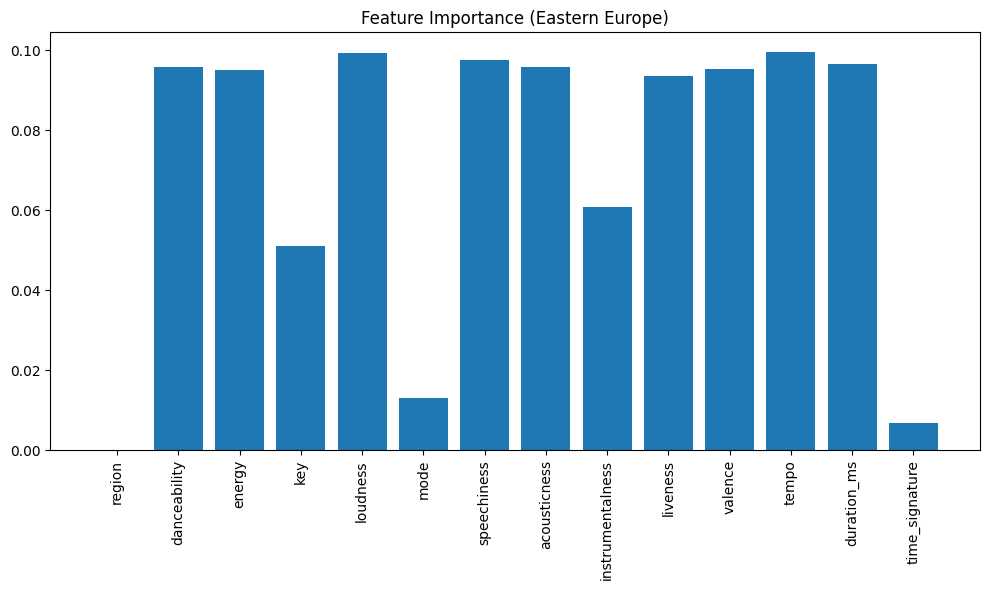
\includegraphics[width=\linewidth]{media/rf_feature_imp_eastern_europe.png}
        \caption{Feature Importance in Eastern Europe}
    \end{minipage}
\end{figure}
\begin{figure}[h]
    \centering
    \begin{minipage}{0.45\textwidth}
        \centering
        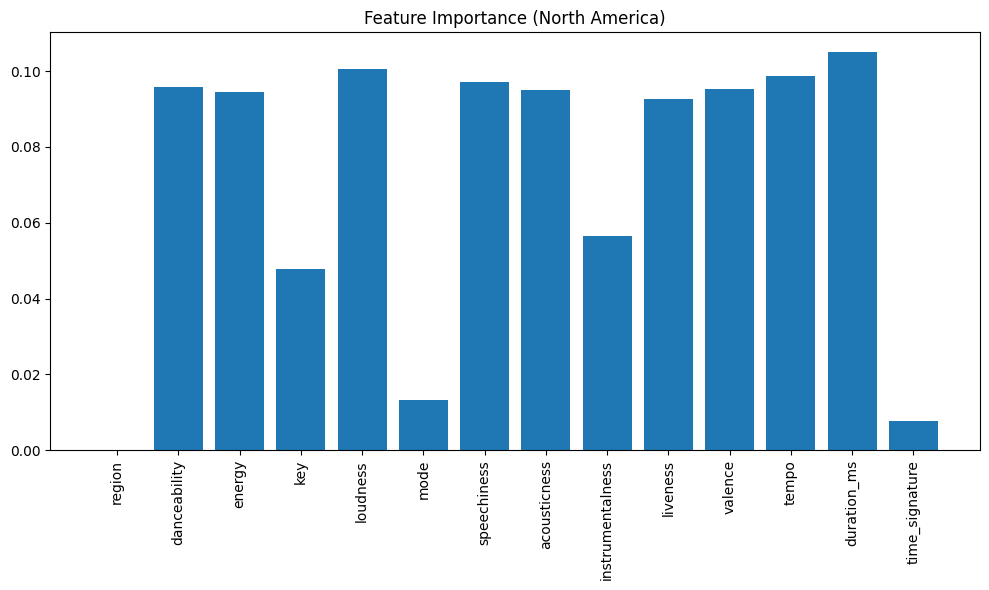
\includegraphics[width=\linewidth]{media/rf_feature_imp_north_america.png}
        \caption{Feature Importance in North America}
    \end{minipage}%
    \hspace{0.05\textwidth} % Space between the two figures
    \begin{minipage}{0.45\textwidth}
        \centering
        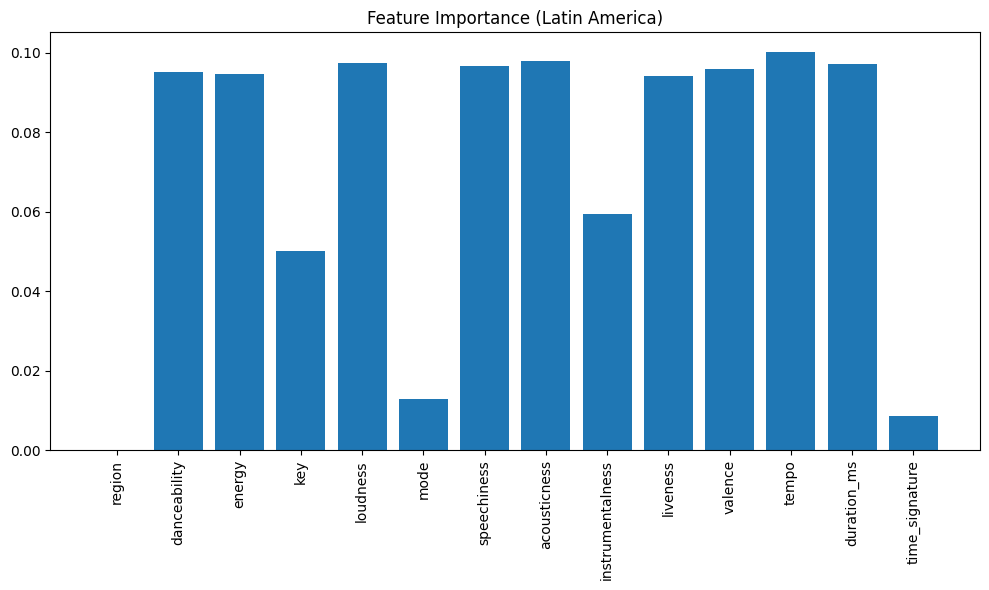
\includegraphics[width=\linewidth]{media/rf_feature_imp_latin_america.png}
        \caption{Feature Importance in Latin America}
    \end{minipage}
\end{figure}
\begin{figure}[h]
    \centering
    \begin{minipage}{0.45\textwidth}
        \centering
        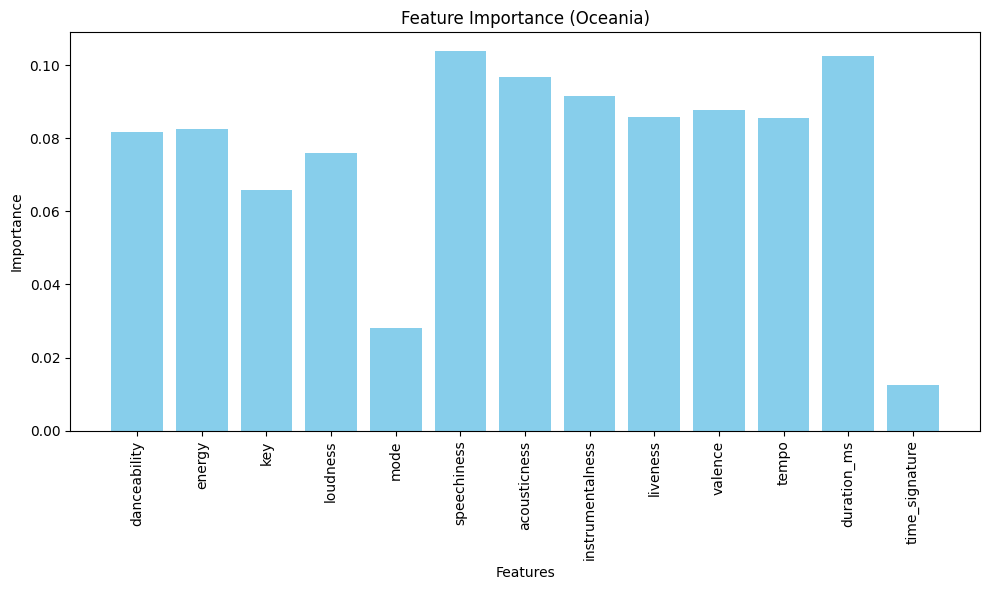
\includegraphics[width=\linewidth]{media/rf_feature_imp_ocenia.png}
        \caption{Feature Importance in Oceania}
    \end{minipage}%
    \hspace{0.05\textwidth} % Space between the two figures
    \begin{minipage}{0.45\textwidth}
        \centering
        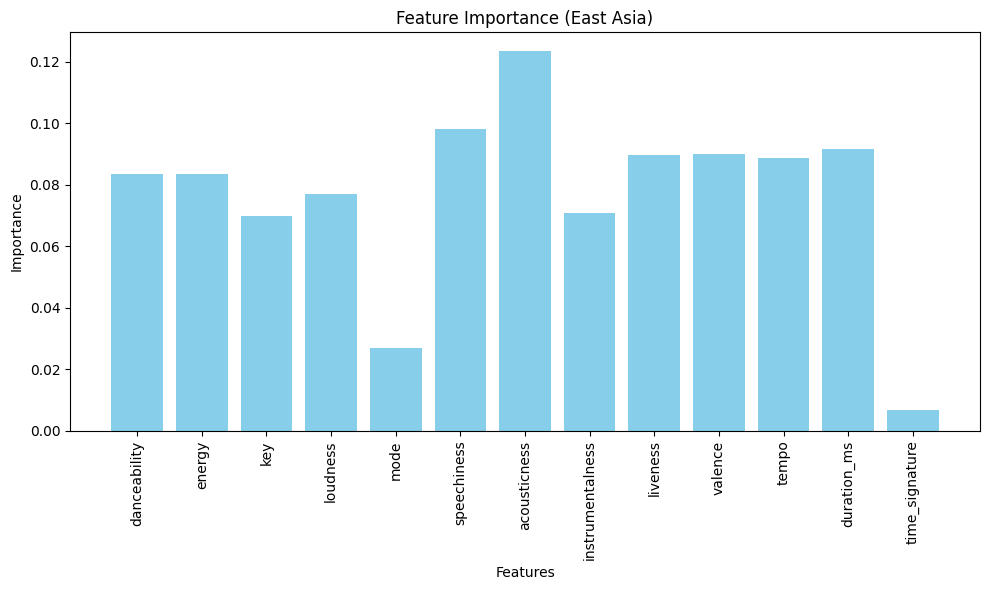
\includegraphics[width=\linewidth]{media/rf_feature_imp_east_asia.png}
        \caption{Feature Importance in East Asia}
    \end{minipage}
\end{figure}
\begin{figure}[h]
    \centering
    \begin{minipage}{0.45\textwidth}
        \centering
        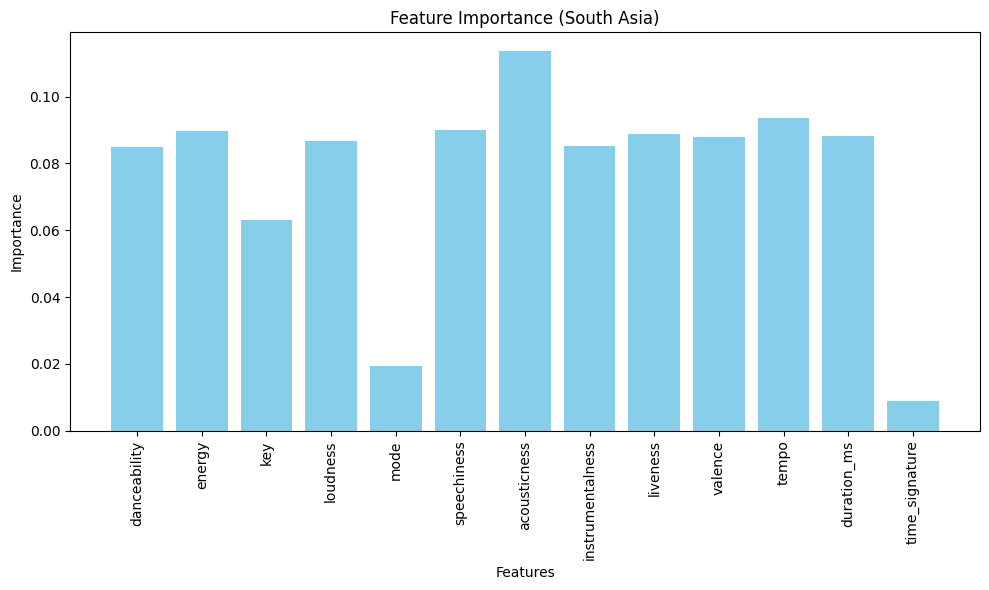
\includegraphics[width=\linewidth]{media/rf_feature_imp_south_asia.png}
        \caption{Feature Importance in South Asia}
    \end{minipage}%
    \hspace{0.05\textwidth} % Space between the two figures
    \begin{minipage}{0.45\textwidth}
        \centering
        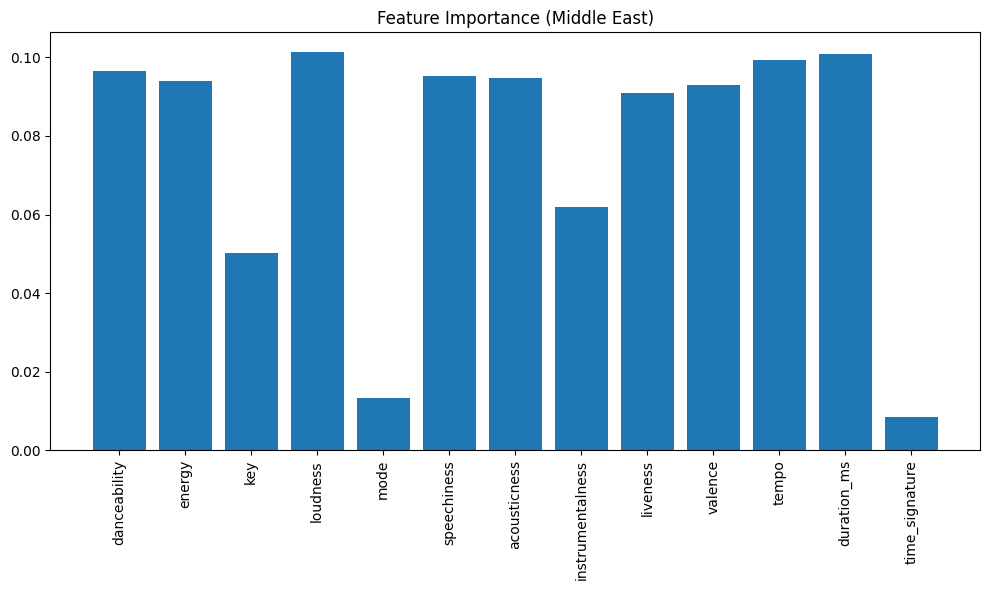
\includegraphics[width=\linewidth]{media/rf_feature_imp_middle_east.png}
        \caption{Feature Importance in Middle East}
    \end{minipage}
\end{figure}
\begin{figure}[h]
    \centering
    \begin{minipage}{0.45\textwidth}
        \centering
        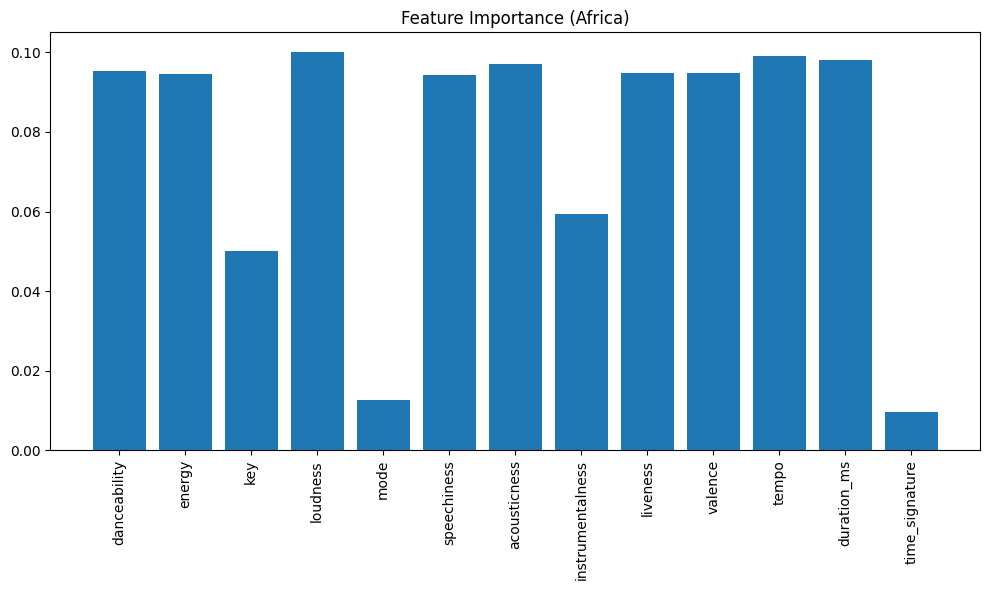
\includegraphics[width=\linewidth]{media/rf_feature_imp_africa.png}
        \caption{Feature Importance in Africa}
    \end{minipage}
\end{figure}

\clearpage 

\textbf{Important Features for Each Region and Their Mean Values:}

Region: Latin America (Code 3)\\
Feature: tempo - Mean Value: 122.61

Region: East Asia (Code 1)\\
Feature: loudness - Mean Value: -6.86\\
Feature: tempo - Mean Value: 121.52\\
Feature: duration\_ms - Mean Value: 229571.73

Region: Eastern Europe (Code 2) \\
Feature: tempo - Mean Value: 122.332345

Region: Middle East (Code 4) \\
Feature: duration\_ms - Mean Value: 213894.57

Region: North America (Code 5) \\
Feature: loudness - Mean Value: -6.99\\
Feature: duration\_ms -  Mean Value: 206987.98

Region: Northern Europe (Code 6) \\
Feature: duration\_ms - Mean Value: 203514.75

Region: Oceania (Code 7) \\
Feature: duration\_ms - Mean Value: 213396.98

Region: South Asia (Code 8) \\
Feature: loudness - Mean Value: -7.39\\
Feature: duration\_ms - Mean Value: 222230.31

Region: Southern Europe (Code 9) \\
Feature: loudness - Mean Value: -7.02

Region: Western Europe (Code 10) \\
Feature: loudness - Mean Value: -7.26\\
Feature: tempo - Mean Value: 120.90

Region: Africa (Code 0) \\
Feature: loudness - Mean Value: -7.608736\\
Feature: tempo - Mean Value: 120.407525
